% !TeX spellcheck = en_GB
\documentclass[12pt]{beamer}

\usetheme[sectionpage=none]{metropolis}
\usepackage{appendixnumberbeamer}

\usepackage{booktabs}
\usepackage{pgfplots}
\usepgfplotslibrary{dateplot}

\usepackage{xspace}
\newcommand{\themename}{\textbf{\textsc{Hard Disk Drive}}\xspace}


% make lists more compact:
\newlength{\wideitemsep}
\setlength{\wideitemsep}{.5\itemsep}
\addtolength{\wideitemsep}{-2pt}
\let\olditem\item
\renewcommand{\item}{\setlength{\itemsep}{\wideitemsep}\olditem}
\renewcommand{\arraystretch}{1.5}

\pretocmd{\tableofcontents}{\begin{minipage}{\textwidth}}{}{}
\apptocmd{\tableofcontents}{\end{minipage}}{}{}

% Presentation metadata
\title{Hard Disk Drives (HDD)}
\subtitle{A technical development journey}
\date{May 10, 2016, Rapperswil}
\author{Cyrill Gsell \& Fabian Hauser}
\institute{Computer Science \\
	TecBEC Presentation FS 2016}

\begin{document}

\maketitle

\begin{frame}{Table of contents}
  \setbeamertemplate{section in toc}[sections numbered]
  \tableofcontents
\end{frame}

\section{Introduction}
\section{What is a Hard Disk Drive?}
\begin{frame}[standout]
	What is a Hard Disk Drive?
\end{frame}
\begin{frame}[fragile]{What is a Hard Disk Drive?}
	\begin{itemize}
		\item \textbf{Data storage!}
		\item How does it work?
			\begin{enumerate}
				\item Logical view
				\item Physical view
			\end{enumerate}
	\end{itemize}
\end{frame}

\begin{frame}[fragile]{What is a Hard Disk Drive: Von Neumann scheme}
	\begin{figure}[p]
		\centering
		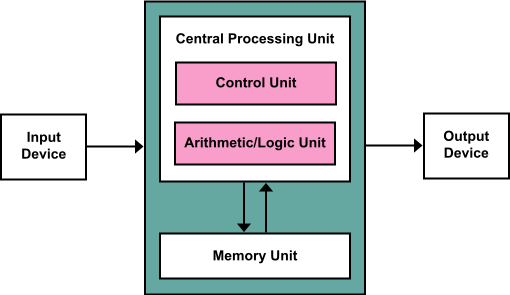
\includegraphics[width=\linewidth]{img/vonneumann.png}
		\caption{CC-BY-SA by Kapooht, Wikipedia}
	\end{figure}
\end{frame}

\begin{frame}[fragile]{What is a Hard Disk Drive: Logical View}
 \begin{columns}[c]
 	\begin{column}[c]{.5\textwidth}
 		\begin{figure}[p]
 			\centering
 			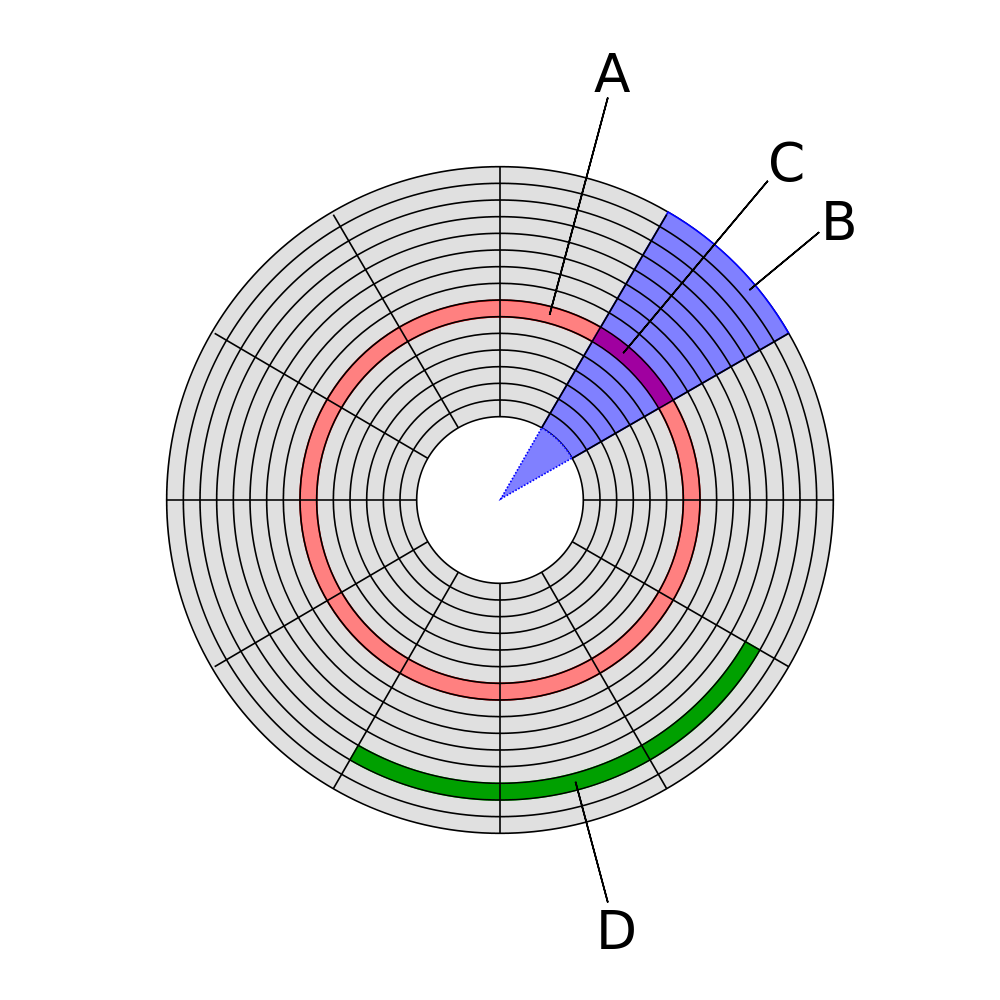
\includegraphics[width=\linewidth]{img/logical.png}
 			\caption{CC0, Wikipedia}
 		\end{figure}
 	\end{column}
 	\begin{column}[c]{.5\textwidth}
 		\begin{description}
	 		\item[A] Track
	 		\item[B] Sector
	 		\item[C] Sector of track
	 		\item[D] Cluster of sectors
		\end{description}
 	\end{column}
 \end{columns}
\end{frame}

\begin{frame}[fragile]{What is a Hard Disk Drive: Physical View}
 \begin{columns}[c]
   	\begin{column}[c]{.4\textwidth}
   		\begin{figure}[p]
   			\centering
   			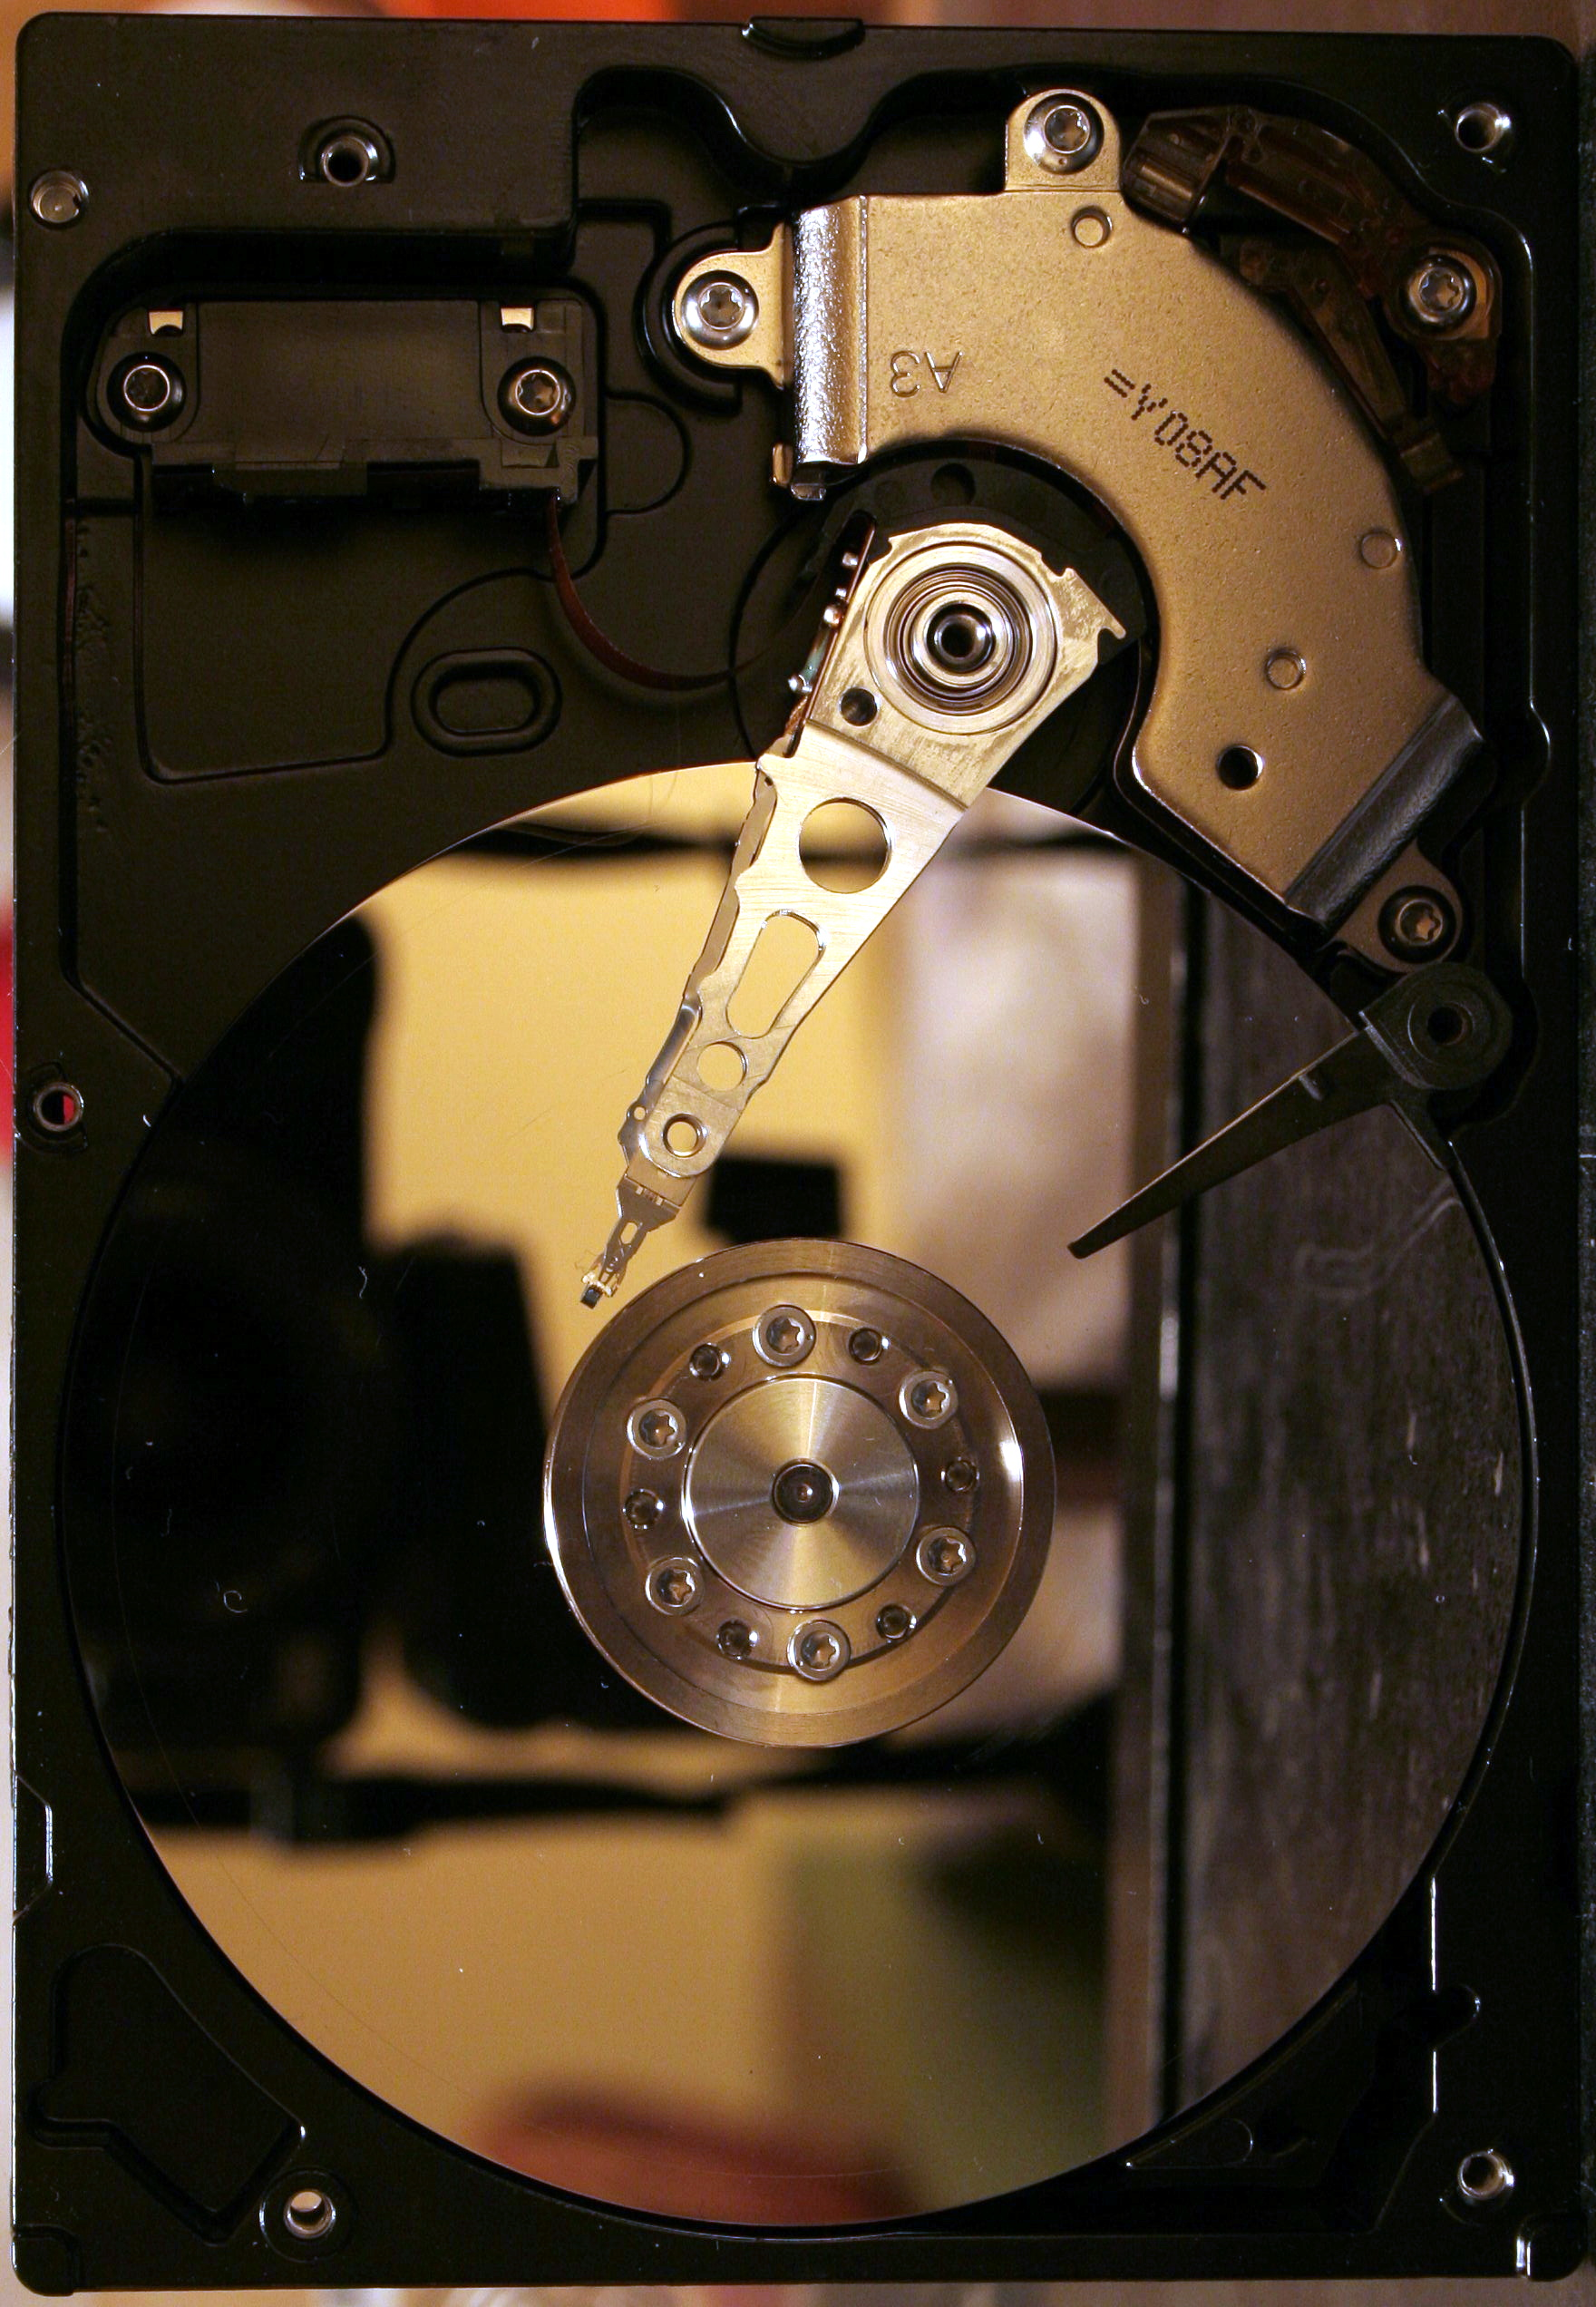
\includegraphics[width=\linewidth]{img/hdd_open.jpg}
   			\caption{CC0,Wikipedia}
   		\end{figure}
   	\end{column}
   	\begin{column}[c]{.6\textwidth}
   		\begin{itemize}
   			\item Rotating disk: usually 7200 rpm
   			\item Writing and reading Head
   			\item Magnet
   			\item Electronics
   		\end{itemize}
   	\end{column}
 \end{columns}
\end{frame}

\begin{frame}[fragile]{What is a Hard Disk Drive: Magnetism}
	Bit encoding / Magnetic structure
	\begin{figure}[p]
		\centering
		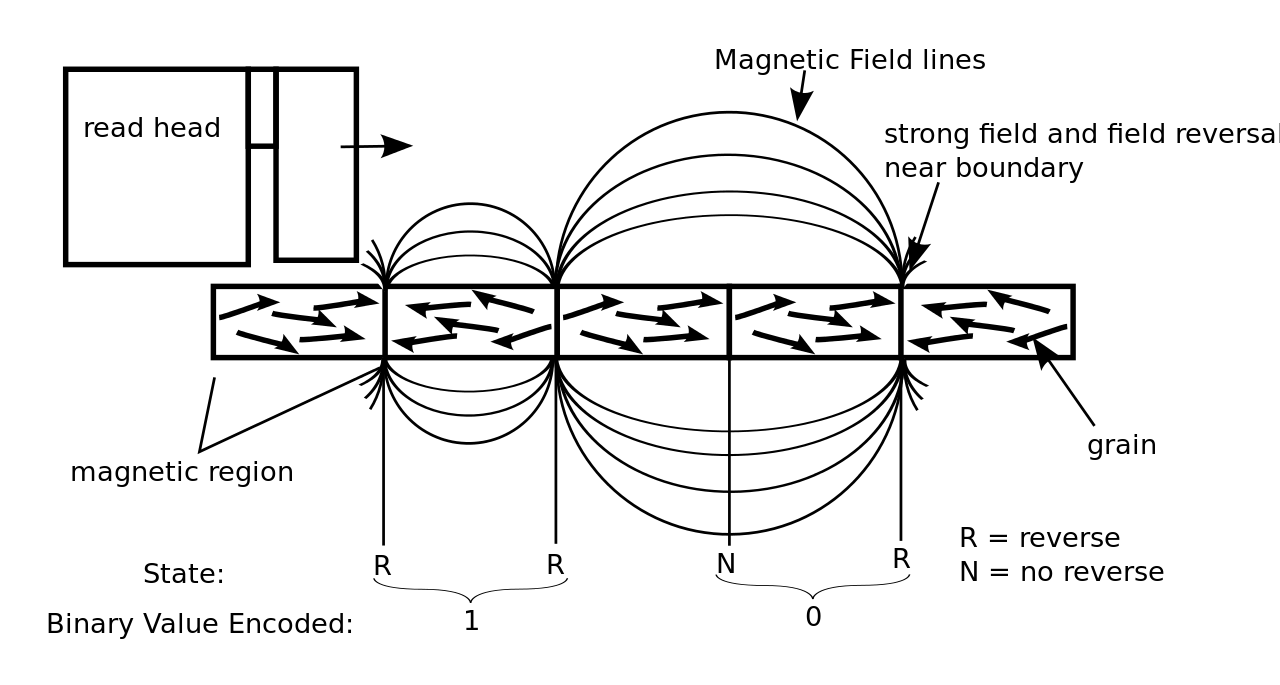
\includegraphics[width=\linewidth]{img/magnetic_track.png}
		\caption{CC-BY-SA Allan Haldane, Wikipedia}
	\end{figure}
\end{frame}

\begin{frame}[fragile]{What is a Hard Disk Drive: Magnetism}
	Magnetic structures
\begin{figure}[p]
	\centering
	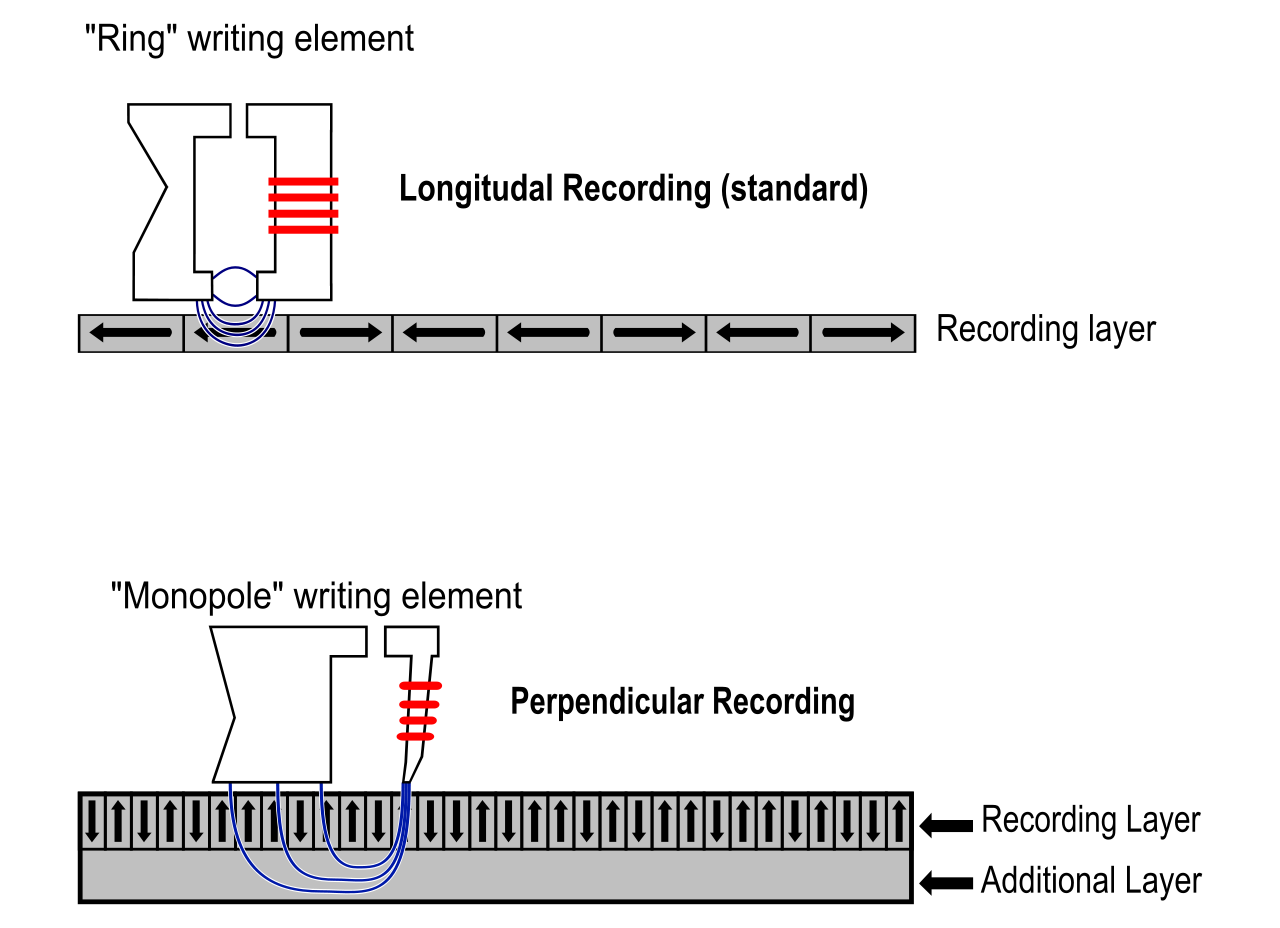
\includegraphics[width=0.75\linewidth]{img/magnetic_type.png}
	\caption{CC0, Wikipedia}
\end{figure}
\end{frame}

\begin{frame}[fragile]{What is a Hard Disk Drive: Physical View}
	Magnetic structure: close up
	\begin{figure}[p]
		\centering
		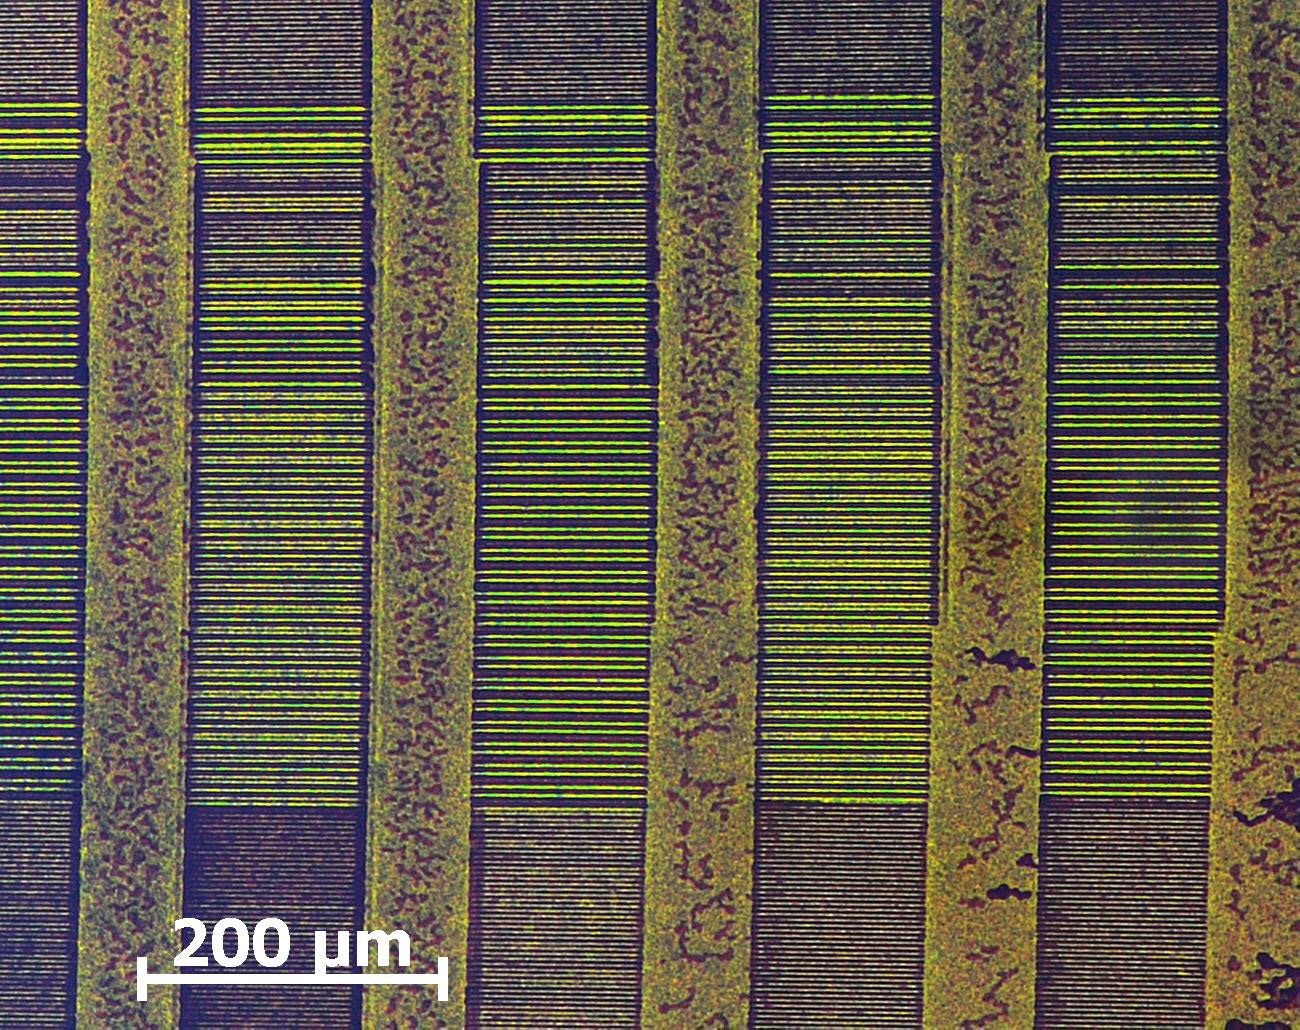
\includegraphics[width=0.7\linewidth]{img/floppy_physical.jpg}
		\caption{CC-BY-SA Matesy GmbH, Wikipedia}
	\end{figure}
\end{frame}

\section{...but why can't we keep floppy disks?}
\begin{frame}[standout]
	...but why can't we keep floppy disks?
\end{frame}
\begin{frame}[fragile]{...but why can't we keep floppy disks?}
	
	 \begin{columns}[c]
	 	\begin{column}[c]{.5\textwidth}
	 		\begin{figure}[p]
	 			\centering
	 			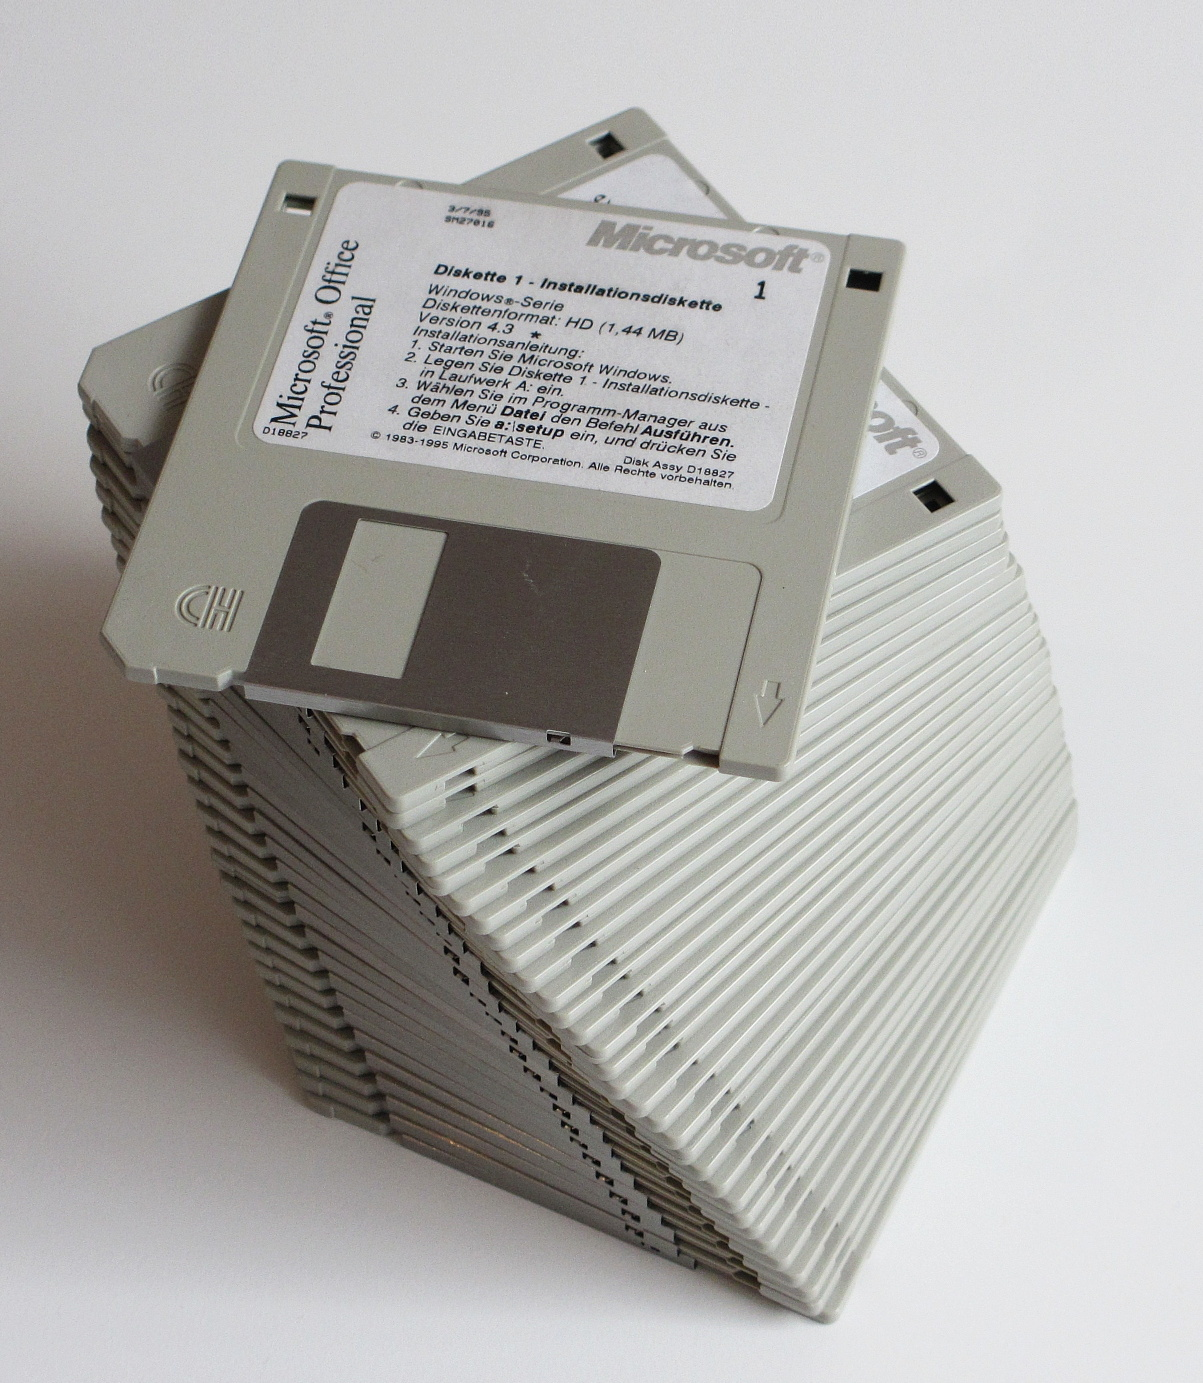
\includegraphics[width=\linewidth]{img/floppy_ms_office_crop.jpg}
	 			\caption{GFDL, JP, Wikipedia}
	 		\end{figure}
	 	\end{column}
	 	\begin{column}[c]{.5\textwidth}
	 		HDDs are better considering:
	 		\begin{itemize}
	 			\item Capacity
	 			\item Durability
	 			\item Price
	 			\item Efficiency / Speed
	 		\end{itemize}
	 		
		 	\hfill
		 	
		 	(CD-ROM and USB-Sticks for portable applications.)
	 	\end{column}
	 \end{columns}
\end{frame}

\section{Evolution}
\begin{frame}[standout]
	Evolution
\end{frame}
\begin{frame}[fragile]{Evolution: First attempts}

	Considering technologies at IBM research center, such as:
	\begin{itemize}
		\item wire matrices
		\item rod arrays
		\item drums / drum arrays
	\end{itemize}
\end{frame}

\begin{frame}[fragile]{Evolution: IBM 350}
	\begin{columns}[c]
	\begin{column}[c]{.5\textwidth}	
 		\begin{figure}[c]
	 		\centering
	 		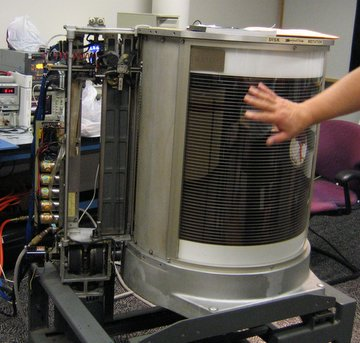
\includegraphics[width=\linewidth]{img/ibm_350.jpg}
	 			\caption{CC BY-SA, Wikipedia}
 		\end{figure}
 	\end{column}
 	
	\begin{column}[c]{.5\textwidth}
		\textbf{1956} IBM 350 Disk File (IBM 305 RAMAC Computer)
	\end{column}
	\end{columns}
\end{frame}

\begin{frame}[fragile]{Evolution: IBM 1301}
	\begin{columns}[c]
	\begin{column}[c]{.5\textwidth}	
 		\begin{figure}[c]
	 		\centering
	 		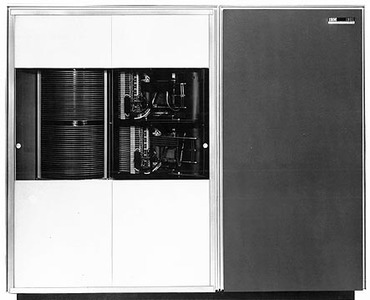
\includegraphics[width=\linewidth]{img/ibm_1301.jpg}
	 			\caption{ibm.com}
 		\end{figure}
 	\end{column}
 	
	\begin{column}[c]{.5\textwidth}
		\textbf{1961} IBM 1301 Disk Storage Unit
	\end{column}
	\end{columns}
\end{frame}

\begin{frame}[fragile]{Evolution: IBM 1311}
	\begin{columns}[c]
	\begin{column}[c]{.5\textwidth}	
 		\begin{figure}[c]
	 		\centering
	 		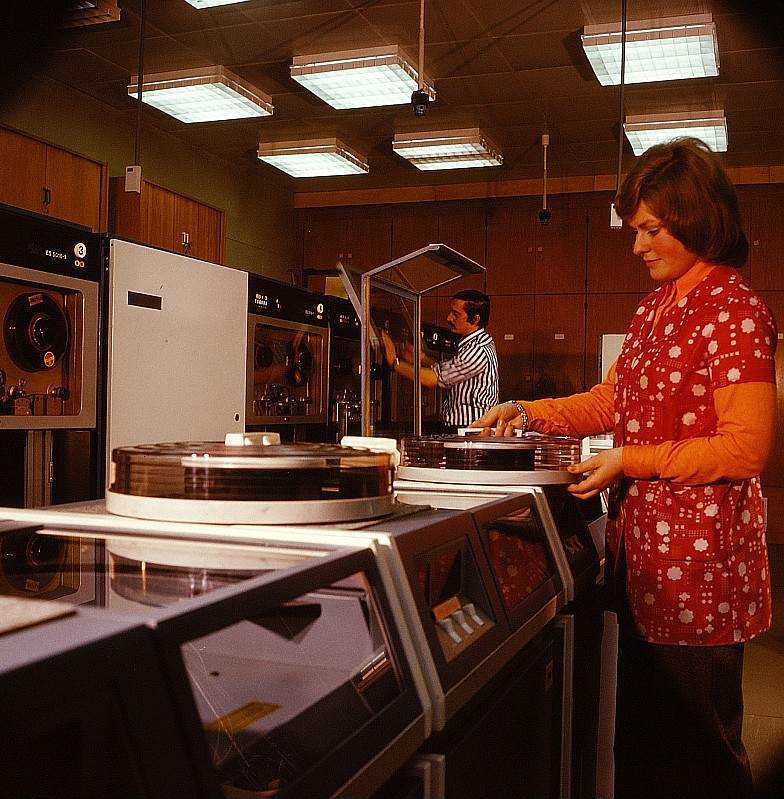
\includegraphics[width=\linewidth]{img/ibm_1311.jpg}
	 			\caption{CC BY-SA, Eugen Nosko, Wikipedia}
 		\end{figure}
 	\end{column}
 	
	\begin{column}[c]{.5\textwidth}
		\textbf{1961} IBM 1311 first disk drive using removable media
	\end{column}
	\end{columns}
\end{frame}

\begin{frame}[fragile]{Evolution: IBM 3340 Winchester}
	\begin{columns}[c]
	\begin{column}[c]{.5\textwidth}	
 		\begin{figure}[c]
	 		\centering
	 		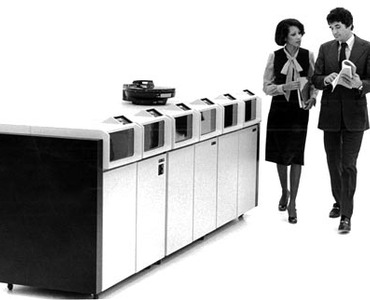
\includegraphics[width=\linewidth]{img/ibm_3340.jpg}
	 			\caption{ibm.com}
 		\end{figure}
 	\end{column}
 	
	\begin{column}[c]{.5\textwidth}
		\textbf{1961} IBM 3340 "Winchester"
	\end{column}
	\end{columns}
\end{frame}

\begin{frame}[fragile]{Evolution: Development, PC era}
	\begin{description}
		\item[early 1980] rare and very expensive optional feature for PC's
		\item[late 1980] standard on PC
		\item[1988] 	HDDs continued getting smaller (introducing 3.5-inch form factor)
		\item[1985] 75 active manufacturers (Industry participation peaked)
		\item[1999] industry participants declined to 15
		\item[2009] 6 remaining
		\item[2012] 3 remaining
	\end{description}
\end{frame}


\begin{frame}[fragile]{Evolution: State of the art}
	\begin{itemize}
		\item TODO!
	\end{itemize}
\end{frame}

\begin{frame}[fragile]{Industry Development}

	\begin{columns}[c]
	\begin{column}[c]{.5\textwidth}	
 		\begin{figure}[p]
	 		\centering
	 		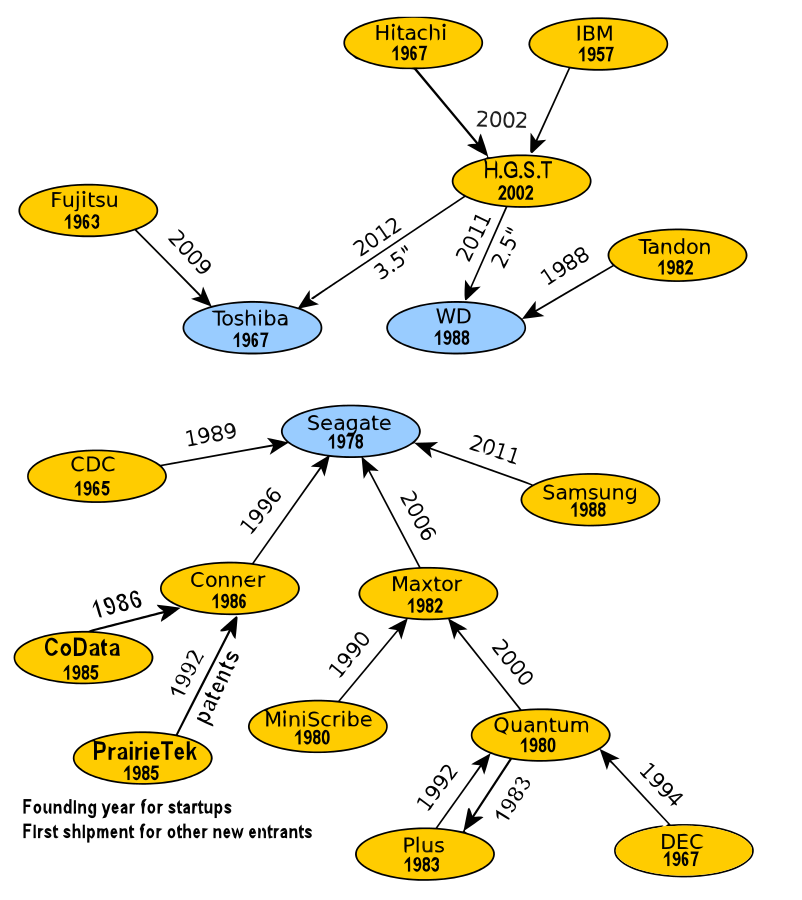
\includegraphics[width=\linewidth]{img/diagram_manufacturer.png}
	 			\caption{CC BY-SA, AUTHOR, Wikipedia}
 		\end{figure}
 	\end{column}
 	
 	\begin{column}[c]{.5\textwidth}	
 		\begin{description}
 			\item[1985] 75 active manufacturers (Industry participation peaked)
			\item[1999] industry participants declined to 15
			\item[2009] 6 remaining
			\item[2012] 3 remaining
 		\end{description}
 	\end{column}
 	\end{columns}
 	
\end{frame}

\section{A glance into the future}
\begin{frame}[standout]
	A glance into the future
\end{frame}
\begin{frame}[fragile]{A glance into the future}
	\begin{itemize}
		\item	In many areas superseded with SSDs / flash storage
		\item	SSHD: SSD and HDD combined \\
				$\rightarrow$ good price \& capacity
		\item	Physical storage density limit: $\approx75$nm tracks. \\
			Work arounds:
			\begin{itemize}
				\item	Helium filling
				\item	Heat assistance (microwave)
				\item	Shingle Magnetic Recording \emph{(SMR)}
				\item	Two-Dimensional Magnetic Recording \emph{(TDMR)}
			\end{itemize}
	\end{itemize}
\end{frame}
\note[itemize]{
	\item SMR (Shingle Magnetic Recording) Overlying the tracks
	\item TDMR (Two-Dimensional Magnetic Recording)
}

\begin{frame}[fragile]{A glance into the future: SMR}
	\begin{figure}[p]
		\centering
		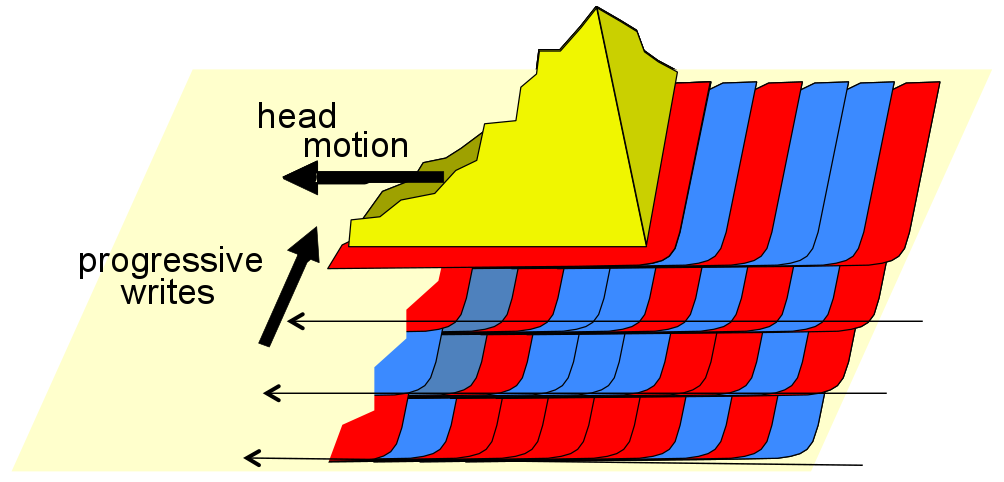
\includegraphics[width=1\linewidth]{img/smr.png}
		\caption{Wood, Williams et al., 2009}
	\end{figure}
\end{frame}

\begin{frame}[fragile]{A glance into the future: TDMR}
	\begin{figure}[p]
		\centering
		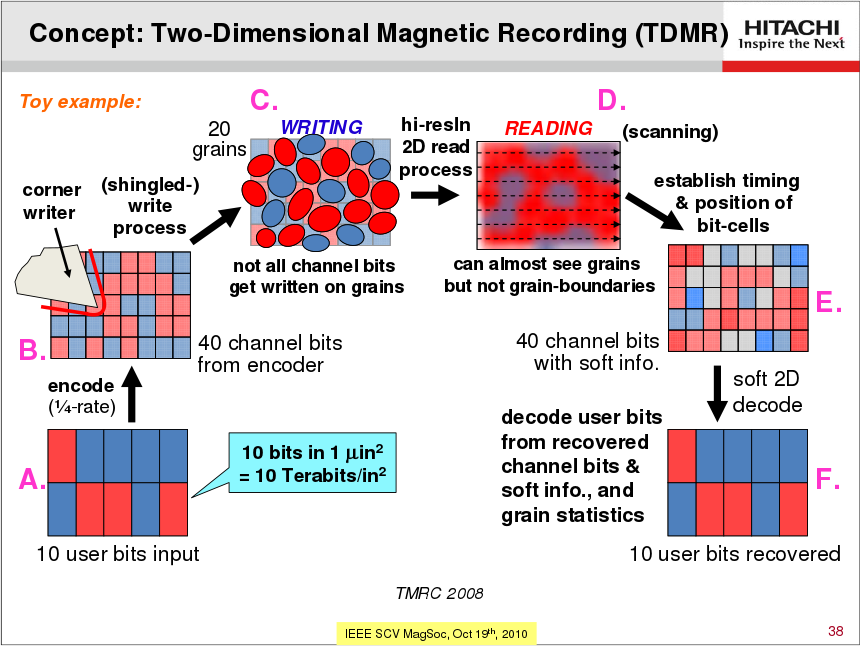
\includegraphics[width=0.85\linewidth]{img/hdd_2d_slides.png}
		\caption{Hitatchi et al., 2010}
	\end{figure}
\end{frame}

\section{Questions}
\begin{frame}[standout]
	Questions? \\
	Thank you for your interest!
\end{frame}

\begin{frame}[fragile]{Ressources}
	\begin{itemize}
		\item \url{http://www.ewh.ieee.org/r6/scv/mag/MtgSum/Meeting2010_10_Presentation.pdf}
		\item \url{https://events.linuxfoundation.org/sites/events/files/slides/SMR-LinuxConUSA-2014.pdf}
	\end{itemize}
\end{frame}


\end{document}
